\begin{frame}
	\frametitle{Answer Set Programming}

	\begin{itemize}
		\item<1-> Paradigma enfocado a la \textcolor{UDCpink}{resolución declarativa} de problemas con complejidad \textcolor{UDCpink}{\textit{NP-hard}}.
		
		\vspace{0.5em}
		
		\item<2-> Combina un \textcolor{UDCpink}{lenguaje simple} con el que modelar problemas lógicos y \textcolor{UDCpink}{herramientas de alto rendimiento}.
	\end{itemize}

	\vspace{1em}
	
	\pause[3]
	
	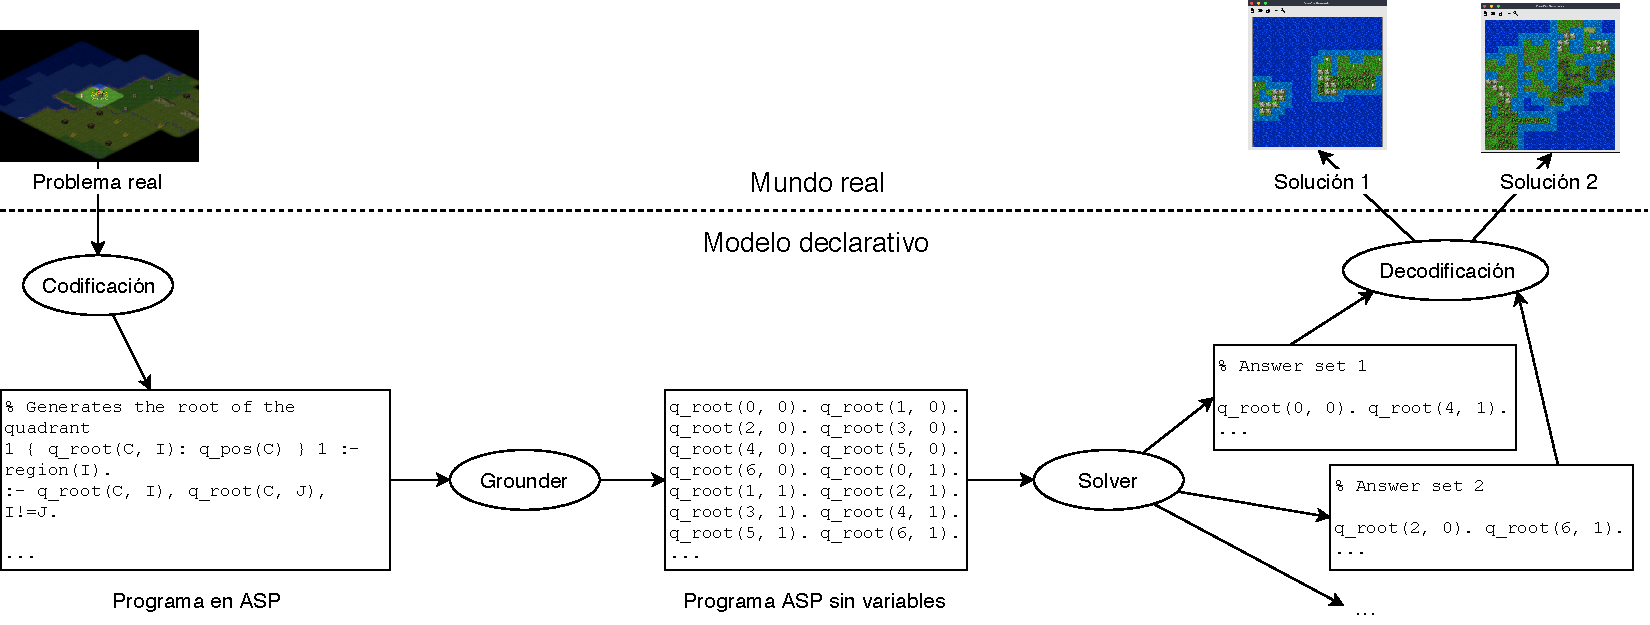
\includegraphics[width=\textwidth]{images/funcionamiento-asp.pdf}
	
\end{frame}

\begin{frame}
	\frametitle{Ejemplo de reglas lógicas}
	
	\begin{block}{Generación del cuadrantes}
	\vspace{1em}
	\hspace{2em}\texttt{1 \{ q\_root(C, I): q\_pos(C) \} 1 :- region(I).}
	
	\hspace{2em}\texttt{:- q\_root(C, I), q\_root(C, J), I!=J.}
	
	\vspace{2em}
	
	\hspace{2em}\texttt{q\_reached(C, I) :- q\_root(C, I).} 
	
	\hspace{2em}\texttt{\{q\_reached(C, I)\} :- q\_reached(D, I), region(I),}
	
	\hspace{4em}\texttt{not existsanother(I, C), q\_adj(D, C).}
	
	\hspace{2em}\texttt{existsanother(I, C) :- q\_reached(C, J), region(J),}
	
	\hspace{4em}\texttt{region(I), J!=I.}
	\vspace{1em}
	\end{block}
	
\end{frame}